% =====================================================================
%  HOLOTRADE — An Exchange for Compute
%  Compile:  C:/Users/wiljd/tools/tectonic/tectonic.exe docs/holotrade.tex --outdir docs
%
%  Written to be read by an investor with no technical background AND by
%  an engineer who wants to check the arithmetic. Every technical term
%  gets a plain-English box the first time it appears. Every number is
%  labelled with how it was obtained: proved, measured, modelled, or
%  published.
% =====================================================================

\documentclass[11pt,letterpaper]{article}

\usepackage[T1]{fontenc}
\usepackage[utf8]{inputenc}
\usepackage{lmodern}
\usepackage[margin=1.05in,top=1.15in,bottom=1.1in]{geometry}
\usepackage{amsmath,amssymb}
\usepackage{booktabs}
\usepackage{array}
\usepackage{longtable}
\usepackage{enumitem}
\usepackage{xcolor}
\usepackage[most]{tcolorbox}
\usepackage{tikz}
\usepackage{graphicx}
\usepackage{titlesec}
\usepackage{fancyhdr}
\usepackage{microtype}
\usepackage{multicol}
\usepackage[hidelinks]{hyperref}

\usetikzlibrary{arrows.meta,positioning,fit,backgrounds,calc,shapes.geometric,decorations.pathreplacing}

% ---------- palette ----------
\definecolor{ink}{HTML}{101B2D}
\definecolor{navy}{HTML}{15304F}
\definecolor{cyan}{HTML}{0E7FA8}
\definecolor{cyanlite}{HTML}{E4F2F8}
\definecolor{amber}{HTML}{A8730E}
\definecolor{amberlite}{HTML}{FBF3E3}
\definecolor{green}{HTML}{1F7A5C}
\definecolor{greenlite}{HTML}{E6F3EE}
\definecolor{red}{HTML}{A32F3E}
\definecolor{redlite}{HTML}{FAEDEF}
\definecolor{grey}{HTML}{5D6B80}
\definecolor{greylite}{HTML}{F2F4F7}
\definecolor{rule}{HTML}{C8D2E0}

\hypersetup{colorlinks=true,linkcolor=cyan,urlcolor=cyan,citecolor=cyan}

% ---------- typography ----------
\titleformat{\section}
  {\normalfont\Large\bfseries\color{navy}}{\thesection}{0.8em}{}
\titleformat{\subsection}
  {\normalfont\large\bfseries\color{cyan!75!black}}{\thesubsection}{0.7em}{}
\titleformat{\subsubsection}
  {\normalfont\normalsize\bfseries\color{ink}}{\thesubsubsection}{0.6em}{}
\titlespacing*{\section}{0pt}{16pt}{7pt}
\titlespacing*{\subsection}{0pt}{12pt}{5pt}

\pagestyle{fancy}
\fancyhf{}
\renewcommand{\headrulewidth}{0.4pt}
\renewcommand{\headrule}{\hbox to\headwidth{\color{rule}\leaders\hrule height \headrulewidth\hfill}}
\lhead{\footnotesize\color{grey}\textsc{Holotrade}\ \ \textbar\ \ An Exchange for Compute}
\rhead{\footnotesize\color{grey}\thepage}

\setlength{\parskip}{5pt}
\setlength{\parindent}{0pt}

% ---------- boxes ----------
\newtcolorbox{plainbox}[1][]{
  enhanced, breakable,
  colback=cyanlite, colframe=cyan,
  boxrule=0pt, leftrule=2.6pt, arc=1.5pt,
  left=9pt,right=9pt,top=7pt,bottom=7pt,
  fonttitle=\bfseries\footnotesize\sffamily,
  coltitle=cyan!60!black,
  title={IN PLAIN ENGLISH\ifx\relax#1\relax\else: #1\fi},
  attach boxed title to top left={yshift=-2pt,xshift=9pt},
  boxed title style={colback=cyanlite,boxrule=0pt,sharp corners}
}

\newtcolorbox{keybox}[1]{
  enhanced, breakable,
  colback=white, colframe=navy,
  boxrule=1pt, arc=2pt,
  left=11pt,right=11pt,top=9pt,bottom=9pt,
  fonttitle=\bfseries\small\sffamily, coltitle=white,
  colbacktitle=navy,
  title={#1}
}

\newtcolorbox{scopebox}{
  enhanced, breakable,
  colback=greylite, colframe=grey,
  boxrule=0pt, leftrule=2.6pt, arc=1.5pt,
  left=9pt,right=9pt,top=7pt,bottom=7pt,
  fontupper=\small
}

\newtcolorbox{warnbox}[1][Worth being careful about]{
  enhanced, breakable,
  colback=amberlite, colframe=amber,
  boxrule=0pt, leftrule=2.6pt, arc=1.5pt,
  left=9pt,right=9pt,top=7pt,bottom=7pt,
  fonttitle=\bfseries\footnotesize\sffamily, coltitle=amber!60!black,
  title={#1},
  attach boxed title to top left={yshift=-2pt,xshift=9pt},
  boxed title style={colback=amberlite,boxrule=0pt,sharp corners}
}

\newtcolorbox{resultbox}[1]{
  enhanced, breakable,
  colback=greenlite, colframe=green,
  boxrule=0pt, leftrule=2.6pt, arc=1.5pt,
  left=9pt,right=9pt,top=7pt,bottom=7pt,
  fonttitle=\bfseries\footnotesize\sffamily, coltitle=green!55!black,
  title={#1},
  attach boxed title to top left={yshift=-2pt,xshift=9pt},
  boxed title style={colback=greenlite,boxrule=0pt,sharp corners}
}

% evidence tags
\newcommand{\tagbox}[3]{\tikz[baseline=(X.base)]{\node[inner xsep=3.5pt,inner ysep=1.4pt,rounded corners=1.6pt,fill=#1,text=#2,font=\bfseries\sffamily\tiny] (X) {#3};}}
\newcommand{\PROVED}{\tagbox{greenlite}{green!45!black}{PROVED}}
\newcommand{\MEASURED}{\tagbox{cyanlite}{cyan!55!black}{MEASURED}}
\newcommand{\MODELLED}{\tagbox{amberlite}{amber!55!black}{MODELLED}}
\newcommand{\PUBLISHED}{\tagbox{greylite}{grey}{PUBLISHED}}

\newcommand{\bignum}[2]{{\color{navy}\bfseries\Large #1}\,{\footnotesize\color{grey}#2}}
\newcommand{\W}{\ensuremath{W(3,3)}}

\begin{document}

% =====================================================================
% TITLE
% =====================================================================
\thispagestyle{empty}
\begin{center}
\vspace*{0.2cm}


\begin{tikzpicture}[scale=1]
  \node[circle,draw=cyan,line width=2.6pt,minimum size=1.5cm] (c) {};
  \fill[cyan] (c.center) circle (3.2pt);
  \foreach \a in {30,90,...,330}{
    \fill[cyan!45] (\a:0.75) circle (1.9pt);
    \draw[cyan!30,line width=0.5pt] (c.center) -- (\a:0.75);
  }
\end{tikzpicture}

\vspace{0.35cm}
{\color{navy}\fontsize{40}{44}\selectfont\bfseries HOLOTRADE}

\vspace{0.28cm}
{\color{cyan}\Large An Exchange for Compute}

\vspace{0.15cm}
{\color{grey}\large Node-seconds priced on live energy, node genetics,\\ hardware health, and fabric coherence}

\vspace{1.0cm}
{\color{rule}\rule{0.55\textwidth}{0.7pt}}
\vspace{0.7cm}

\begin{minipage}{0.86\textwidth}
\centering\itshape\color{ink}
Every compute marketplace in existence sells the same product: a rectangle of
capacity for a span of time. That product is a billing artefact --- it exists
because provisioning used to take minutes. When the unit boots in 171
milliseconds, the hour has no physical justification left, and everything
interesting about a machine that the hour was flattening becomes priceable.

\vspace{5pt}
This paper is about what becomes priceable.
\end{minipage}

\vspace{1.1cm}
{\color{rule}\rule{0.55\textwidth}{0.7pt}}

\vspace{0.9cm}
{\large\bfseries Wil Dahn}\\[2pt]
{\color{grey}\normalsize Built on the \W--E$_8$ substrate programme}\\[3pt]
{\color{grey}\small\texttt{github.com/wilcompute/Holotrade}}

\vspace{0.9cm}
{\color{grey}\small August 2026}

\vfill
\begin{minipage}{0.9\textwidth}
\footnotesize\color{grey}
\textbf{How to read the evidence tags.} Every headline figure in this document
carries one. \PROVED\ means finite mathematics with a machine-checkable proof
in the repository. \MEASURED\ means it came out of a run you can reproduce with
\texttt{npm test}. \MODELLED\ means it is a simulation parameter or an estimate,
and is never presented as a measurement. \PUBLISHED\ means it is somebody
else's result and is cited as such. Where a figure does not survive scrutiny,
the correction stays on the page beside it.
\end{minipage}
\vspace{0.4cm}
\end{center}

\newpage

% =====================================================================
\tableofcontents
\newpage

% =====================================================================
\section{The thesis, in one page}

Compute is the largest new commodity of the century and it is being sold with
the crudest possible pricing model: a fixed hourly rate for an
undifferentiated box. That model destroys information in four directions at
once.

\begin{enumerate}[leftmargin=1.4em,itemsep=4pt]
\item \textbf{It destroys the energy signal.} Wholesale electricity prices move
every five minutes and go negative overnight in Texas. An hourly rate cannot
express that, so the operator eats the volatility and prices in a margin to
survive it. The buyer pays that margin whether or not the volatility happened.

\item \textbf{It destroys the machine's history.} Two identical servers that
have run different work for a month are no longer the same product. One of them
already carries statistical priors for the job you are about to run and will
finish in fewer hours. Nobody prices that, because an hourly rate has no place
to put it.

\item \textbf{It destroys the wear signal.} A machine everybody wants is a
machine wearing out faster than its neighbours, and a machine nobody wants is
still aging, still drawing standby power, and still due for the same service
visit. A single rate charges both the same and balances neither.

\item \textbf{It destroys the shape.} Forty machines scattered across a
datacentre and forty machines wired as one coherent block are sold as the same
forty machines. They are not remotely the same thing, and the difference ---
bandwidth between them --- is then sold back to you as a separate line item.
\end{enumerate}

Holotrade prices all four. The mechanism is a single multiplicative formula in
which each term is independently observable and shown to the buyer on every
quote:

\begin{center}
\begin{tcolorbox}[enhanced,colback=white,colframe=navy,boxrule=1pt,arc=2pt,width=0.9\textwidth,halign=center]
{\Large $P \;=\; P_0 \times E \times G \times D \times H \times Q \times L$}\\[4pt]
{\footnotesize\color{grey}base $\times$ energy $\times$ genetics $\times$ demand/wear $\times$ health $\times$ quantum $\times$ locality}
\end{tcolorbox}
\end{center}

The unit that formula prices is not an hour. It is the \textbf{node-second},
made possible because a modern microVM boots in about 171 milliseconds
\PUBLISHED{} --- two orders of magnitude below the settlement interval, so a
one-second slice is more than 99\% useful work.

\begin{resultbox}{The result that pays for the whole design}
The demand term $D$ is \emph{two-sided}: it charges a premium above a target
utilisation band and pays a discount below it. Run the exchange with that
mechanism on and off, and the Gini coefficient of fleet utilisation --- the
standard measure of how unevenly load is distributed --- falls from
\textbf{0.164} to \textbf{0.083}. \MEASURED

\vspace{4pt}
That is a \textbf{50\% reduction in fleet dispersion}, and it is not decorative.
Thermal cycling, not duty cycle, is what physically destroys silicon. A fleet
whose nodes are evenly loaded cycles less, lasts longer, and produces service
events spread across the calendar instead of arriving in a clump that has to be
staffed for.
\end{resultbox}

Everything else in this paper follows from taking those two moves seriously: a
sub-second unit, and a price with observable parts.

\newpage

% =====================================================================
\section{What is actually being sold}

\subsection{The case against the hour}

Every incumbent sells node-hours. The hour is not a unit of computation; it is a
unit of \emph{scheduling overhead}. It became standard because bringing a
conventional virtual machine into existence takes minutes, and if provisioning
costs you three minutes then billing in anything smaller than an hour is
absurd.

\begin{plainbox}[What a virtual machine is]
A physical server is one piece of hardware. A \emph{virtual machine} is a
software-created illusion of a whole separate computer running on top of it, so
that one physical server can be rented to several customers at once without
them being able to see or interfere with each other. The software that creates
the illusion is called a \emph{hypervisor}. Creating a traditional virtual
machine involves booting a complete operating system inside the illusion, which
is why it takes minutes.
\end{plainbox}

\begin{plainbox}[What a microVM is, and why it changes the economics]
A \emph{microVM} is a stripped-down virtual machine: a real hypervisor
boundary, a real separate operating-system kernel, but with everything
unnecessary for one specific job removed --- no virtual graphics card, no
virtual sound card, no legacy device emulation. It gets the same security
isolation as a full virtual machine in a small fraction of the startup time.
Amazon's \emph{Firecracker} is the best-known implementation and is what runs
their serverless products.
\end{plainbox}

Published measurements put microVM boot at a median of \textbf{171.5\,ms}, with
95\% under 176\,ms and 99\% under 178\,ms, measured on Firecracker over
rotational storage --- a deliberately pessimistic baseline, since production
fleets use flash \PUBLISHED. Once the unit comes into existence in under a fifth
of a second, three things follow immediately.

\begin{enumerate}[leftmargin=1.4em,itemsep=5pt]
\item \textbf{The hour has no physical justification.} A one-second billing
slice carries roughly 17\% startup overhead in the worst case where every
second is a fresh boot, and effectively zero for any job that runs longer than
a few seconds. There is no technical reason to round up to 3{,}600 seconds.

\item \textbf{Per-second energy pricing becomes possible rather than
theatrical.} You cannot price a resource at a granularity finer than your
settlement interval. If you settle hourly, the five-minute grid price is
information you have thrown away before you could act on it.

\item \textbf{The startup cost becomes visible instead of smeared.} Holotrade
charges the boot \emph{once, explicitly, as its own line}, rather than folding
it into the rate. A customer running many short jobs can therefore see exactly
what their fan-out pattern costs them --- which is information the hourly model
structurally cannot provide.
\end{enumerate}

\subsection{Three objects, not one}

\begin{center}
\renewcommand{\arraystretch}{1.5}
\begin{tabular}{@{}p{0.14\textwidth} p{0.20\textwidth} p{0.58\textwidth}@{}}
\toprule
\textbf{Layer} & \textbf{Object} & \textbf{What it is} \\
\midrule
\textsc{asset} & the \textbf{node} &
A durable machine with an identity, an accumulated learning history, and a
physical wear record. This is what you own, lease, or lend into the pool.\\
\textsc{contract} & the \textbf{execution plan} &
A cryptographically signed document naming exactly what will run, against which
software artefacts, with which network permissions, inside which time window.
It exists --- and can be traded --- before anything executes.\\
\textsc{unit} & the \textbf{node-second} &
What actually settles. Metered against the real electricity price at the second
it was drawn.\\
\bottomrule
\end{tabular}
\end{center}

\begin{plainbox}[What an execution plan is, and why it matters commercially]
Think of it as a signed work order. Before any machine starts, the plan states:
here is the exact software (identified by a cryptographic fingerprint, so it
cannot be swapped for something else), here is the only network address it is
permitted to contact, here is the window during which this authorisation is
valid, and here is my signature over all of it.

\vspace{4pt}
Commercially this is the difference between renting a machine and buying a
\emph{guarantee about what happened on it}. It is what lets a bank, a hospital,
or a defence contractor use somebody else's hardware. It is also what makes
compute genuinely tradeable: a signed plan is a contract with a specification,
so it can change hands before it runs, the way a futures contract does.
\end{plainbox}

\subsection{Why isolation is a precondition for the market existing at all}

A two-sided marketplace requires that an owner of idle machines be willing to
run a stranger's code on them. Without hardware-enforced isolation, ``list your
spare capacity'' is a request to be compromised, and the supply side never
materialises.

The isolation model Holotrade assumes is the strong one now standard in this
class of system: each job gets its own operating-system kernel under a real
hypervisor (not a shared kernel, as with containers); the guest has \emph{no
network device at all} by default, with all input and output crossing a single
narrow channel to the host; the filesystem is cryptographically sealed so that
tampering prevents boot rather than being detected afterwards; and every
lifecycle event is written to a hash-chained log \PUBLISHED.

\begin{plainbox}[What a hash chain is]
Each entry in the log includes a fingerprint of the entry before it. Change or
delete any entry and every subsequent fingerprint stops matching --- so
tampering is not merely discouraged, it is arithmetically detectable by anyone
holding the log. It is the same idea that underpins a blockchain, without
needing a blockchain.
\end{plainbox}

\newpage

% =====================================================================
\section{The price, term by term}

The formula is multiplicative rather than additive. That is a deliberate
engineering choice with three consequences: the terms stay independent so each
can be measured on its own; each keeps its own auditable line on the quote; and
because each is separately bounded, no single factor can drag the price to zero
or to infinity by itself.

\begin{center}
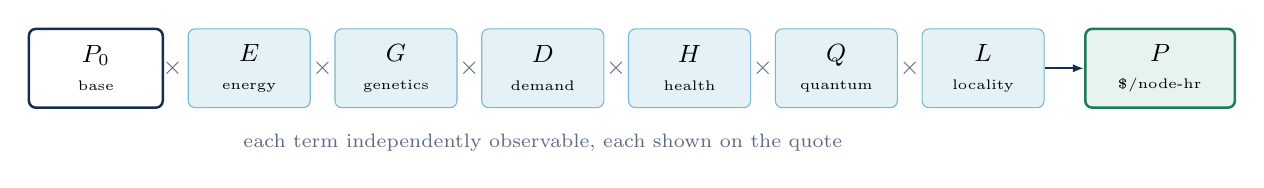
\begin{tikzpicture}[font=\small]
  \tikzset{
    tm/.style={draw=cyan!55,fill=cyanlite,rounded corners=2.5pt,minimum width=1.55cm,minimum height=1.0cm,align=center,inner sep=3pt},
    bs/.style={draw=navy,fill=white,rounded corners=2.5pt,minimum width=1.7cm,minimum height=1.0cm,align=center,line width=0.9pt},
    result/.style={draw=green,fill=greenlite,rounded corners=2.5pt,minimum width=1.9cm,minimum height=1.0cm,align=center,line width=0.9pt},
  }
  \node[bs] (b) {$P_0$\\[-1pt]{\tiny base}};
  \node[tm,right=3mm of b] (e) {$E$\\[-1pt]{\tiny energy}};
  \node[tm,right=3mm of e] (g) {$G$\\[-1pt]{\tiny genetics}};
  \node[tm,right=3mm of g] (d) {$D$\\[-1pt]{\tiny demand}};
  \node[tm,right=3mm of d] (h) {$H$\\[-1pt]{\tiny health}};
  \node[tm,right=3mm of h] (q) {$Q$\\[-1pt]{\tiny quantum}};
  \node[tm,right=3mm of q] (l) {$L$\\[-1pt]{\tiny locality}};
  \node[result,right=5mm of l] (p) {$P$\\[-1pt]{\tiny \$/node-hr}};
  \foreach \a/\b in {b/e,e/g,g/d,d/h,h/q,q/l}{\node at ($(\a)!0.5!(\b)$) {\color{grey}$\times$};}
  \draw[-{Latex[length=4pt]},navy,line width=0.8pt] (l) -- (p);
  \node[below=2mm of d,text=grey,font=\scriptsize] {each term independently observable, each shown on the quote};
\end{tikzpicture}
\end{center}

% ---------------------------------------------------------------
\subsection{$E$ --- energy}

\begin{plainbox}[]
Datacentres buy electricity on a wholesale market where the price changes every
few minutes. In Texas it goes \emph{negative} at three in the morning --- the
grid pays you to consume --- and spikes to four figures during a heat wave. $E$
is the term that passes that reality through to the buyer.
\end{plainbox}

$E$ is deliberately \emph{not} linear in the grid price. A node should not
become worthless when the grid goes negative, nor unsellable when it spikes.
Holotrade applies a power law with exponent 0.55 on the ratio to that site's
baseline, clamped to $[0.62, 2.40]$. That reproduces how operators actually
behave: they pass through most of a normal move and none of a tail. The
adjustment also accounts for \emph{PUE}.

\begin{plainbox}[What PUE is]
Power Usage Effectiveness. For every watt that reaches a computer chip, a
datacentre spends additional watts on cooling, power conversion and lighting.
PUE is the ratio of total facility power to computing power. A PUE of 1.0 would
be perfect; a well-run modern facility is around 1.1, and a hot-climate
facility with mechanical chillers is 1.4 or worse. It is a straight multiplier
on the electricity bill and therefore on the price.
\end{plainbox}

% ---------------------------------------------------------------
\subsection{$G$ --- genetics}

This is the term that makes Holotrade a different product rather than a better
price list.

\begin{plainbox}[]
When a machine runs the same class of work repeatedly, the software layer on it
accumulates useful statistical structure --- cached compilations, tuned kernel
selections, warm model checkpoints, learned scheduling parameters. The industry
already exploits this deliberately: ``warm starts'' and ``checkpoint merging''
are standard practice in machine-learning operations.

\vspace{4pt}
The consequence is that two physically identical servers, after a month of
different work, are \emph{not the same product}. One of them will reach your
target in fewer hours. Nobody prices that today. Holotrade does, and calls the
accumulated structure the node's \emph{genome} because it is inherited when a
machine's software state is copied onto fresh hardware.
\end{plainbox}

$G$ is built from three separately observable quantities, never from a claim:

\begin{itemize}[leftmargin=1.4em,itemsep=3pt]
\item \textbf{Specialisation} on \emph{this specific} workload class --- not a
general capability score. A node with excellent memory-bandwidth
characteristics gets no credit for it on a workload that is compute-bound.
\item \textbf{Realised fitness}: the completion record. Jobs finished versus
jobs failed, weighted by experience depth. Never a manufacturer's specification.
\item \textbf{Provenance depth}: a long lineage of successful forks is evidence
that a software core is genuinely good rather than lucky.
\end{itemize}

\begin{warnbox}[The caveat that goes on every lease quote]
A leased core keeps specialising toward whatever \emph{you} feed it. Over a
90-day lease it will measurably drift toward your workload class and away from
the one it was strongest at when you rented it. You are buying a starting
point, not a frozen asset --- and by the end of a long lease you will have
changed the thing you rented. Holotrade prints the projected drift on the quote
rather than leaving the customer to discover it.
\end{warnbox}

% ---------------------------------------------------------------
\subsection{$D$ --- demand and wear: the balancer}

\begin{plainbox}[]
The obvious way to price demand is one-sided: a busy machine costs more. That is
what surge pricing does, and it leaves the cold half of your fleet earning
nothing while still aging, still drawing standby power, and still due for the
same maintenance visit.

\vspace{4pt}
Holotrade charges a premium above a target band \emph{and pays a discount
below it}. The discount is not generosity. It is cheaper than the alternative,
and the reason is physical.
\end{plainbox}

\begin{keybox}{Why an evenly loaded fleet physically lasts longer}
Semiconductor devices fail predominantly from \emph{thermal cycling}, not from
accumulated running time. Every time a chip heats up and cools down, the
materials in it expand and contract at different rates; solder joints, die
attachments and interconnects accumulate mechanical fatigue with each cycle.
This is standard reliability engineering and is why the failure curve is
modelled with a Weibull distribution whose shape parameter is above 1, meaning
wear-out rather than random failure.

\vspace{5pt}
So a machine held steadily at 70\% load wears \emph{more slowly} than one
swinging between idle and pinned at the same 70\% average. Reducing the
\emph{dispersion} of load across a fleet therefore does three things at once:
it uses the capital better, it extends the physical life of the hardware, and
it spreads service events across the calendar instead of clustering them.
\end{keybox}

\begin{plainbox}[What a Gini coefficient is]
A single number between 0 and 1 measuring how unevenly something is
distributed. Economists use it for income inequality. Here it measures how
unevenly work is distributed across the fleet: 0 would mean every machine
carries exactly the same load, 1 would mean one machine does everything while
the rest sit idle. Lower is better.
\end{plainbox}

\begin{resultbox}{The measured effect, and why it is a finding rather than an animation}
\begin{center}
\begin{tabular}{@{}lcc@{}}
\toprule
& \textbf{Balancer off} & \textbf{Balancer on} \\
\midrule
Utilisation Gini & 0.164 & \textbf{0.083} \\
\bottomrule
\end{tabular}
\end{center}
\vspace{3pt}
\textbf{Nothing in the simulation pushes utilisation toward the band directly.}
A node's demand target is set by its \emph{price} relative to the median of its
own hardware class, and that price was itself computed from its utilisation.
The band is where the feedback loop settles, not where it is aimed. Turn the
balancer off in the running application and the dispersion climbs. \MEASURED
\end{resultbox}

Two engineering details matter for whether this is honest.

\textbf{The comparison set is the hardware class, not the fleet.} A buyer
choosing between accelerators does not consider a general-purpose CPU node
``cheap'' --- they are not substitutes. Comparing against a fleet-wide median
would make every CPU look like a permanent bargain and every scarce node look
permanently extortionate, and the loop would never settle.

\textbf{The curve must be monotone.} If there is any utilisation at which a
node gets \emph{cheaper} by becoming busier, a buyer can arbitrage the discount
by loading the machine they are about to rent. An earlier version of this
design had exactly that defect at one of the seams between the discount, band
and premium regions. It was caught by a monotonicity test, and the test is in
the repository.

\begin{center}
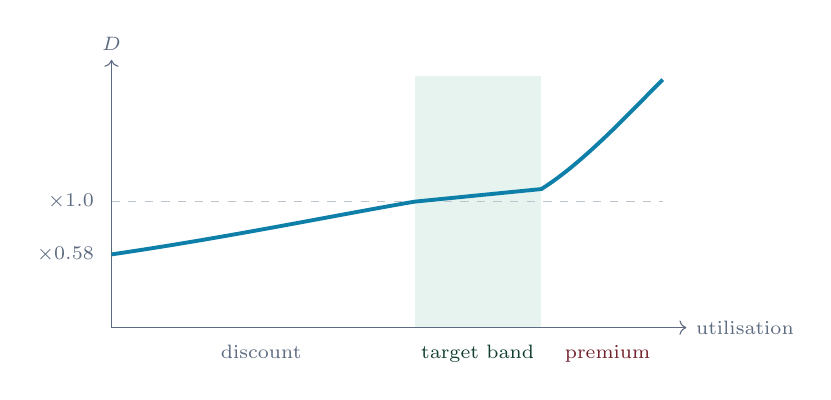
\begin{tikzpicture}[scale=1,font=\footnotesize]
  \fill[greenlite] (3.85,0) rectangle (5.46,3.2);
  \draw[grey!40,dashed] (0,1.6) -- (7,1.6);
  \draw[->,grey] (0,0) -- (7.3,0) node[right,font=\scriptsize] {utilisation};
  \draw[->,grey] (0,0) -- (0,3.4) node[above,font=\scriptsize] {$D$};
  \draw[cyan,line width=1.4pt]
    (0,0.93) .. controls (1.5,1.15) and (2.8,1.42) .. (3.85,1.6)
    -- (5.46,1.76)
    .. controls (6.0,2.1) and (6.6,2.75) .. (7,3.15);
  \node[grey,font=\scriptsize,anchor=north] at (1.9,-0.1) {discount};
  \node[green!50!black,font=\scriptsize,anchor=north] at (4.65,-0.1) {target band};
  \node[red!70!black,font=\scriptsize,anchor=north] at (6.3,-0.1) {premium};
  \node[grey,font=\scriptsize,anchor=east] at (-0.1,1.6) {$\times 1.0$};
  \node[grey,font=\scriptsize,anchor=east] at (-0.1,0.93) {$\times 0.58$};
\end{tikzpicture}
\end{center}

The premium region is superlinear because the wear term is: a node that swings
is accumulating damage faster than a node that is merely busy, and the premium
it earns is the maintenance reserve being funded by the people causing the wear.
That is not arbitrage. It is the correct allocation of a real cost.

% ---------------------------------------------------------------
\subsection{$H$ --- health}

A worn machine delivers less per hour, so it should cost less per hour, and it
should be \emph{visibly} cheaper rather than quietly slower. $H$ multiplies
three observable things: the performance derate you actually receive, a
reliability discount derived from the instantaneous failure hazard, and a drift
term from accumulated correctable memory errors.

\begin{plainbox}[What a correctable error is, and why it predicts failure]
Server memory detects and silently repairs single-bit corruptions. A machine
reporting a rising count of these is not yet failing, but it is a well
established leading indicator that it will. Holotrade treats the count as a
priced signal rather than an alert nobody reads.
\end{plainbox}

% ---------------------------------------------------------------
\subsection{$Q$ --- quantum}

\begin{plainbox}[]
This term is 1 --- exactly, permanently --- for every ordinary workload. It is
included because the underlying architecture makes a sharp distinction between
two kinds of computation, and that distinction turns out to be commercially
useful even for customers who will never buy a quantum anything.
\end{plainbox}

There is a class of operations, called \emph{Clifford} operations, that a
theorem of Gottesman and Knill shows can be simulated on any ordinary computer
in polynomial --- that is, practical --- time \PUBLISHED. On this architecture,
that class covers everything structural: the routing, the memory addressing,
the error correction, the fault tolerance. All of it runs on any hardware
anyone already owns.

What is genuinely scarce is the other kind: \emph{non-Clifford} operations,
sometimes called ``magic''. Each one multiplies the cost of classical
simulation by a factor of 9. At $t=6$ that is 531{,}441; at $t=20$ it is
$1.2\times 10^{19}$, and no classical fleet on Earth can help you.

\begin{keybox}{Why this matters even if you never buy quantum capacity}
It gives the product a knob nobody else has. The \emph{structure} of the system
is free and universal --- every machine can run it. The \emph{power} is a
continuously priced resource. You provision advantage the way you provision
storage: as much as you pay for, on a substrate everyone already runs.

\vspace{5pt}
And the refusal is hard. A workload requiring non-Clifford operations cannot be
served by ordinary hardware \emph{at any price} --- not slowly, not
approximately. Holotrade refuses the order and states the reason rather than
silently substituting something that will not work. That refusal is enforced in
software, tested, and also implemented in the hardware primitive described in
\S\ref{sec:rtl}.
\end{keybox}

% ---------------------------------------------------------------
\subsection{$L$ --- locality}

$L$ prices how far a candidate machine is from where your data already sits.
Every provider gestures at this with ``availability zones'', which are
administrative labels rather than measurements. Here it is an exact distance,
and \S\ref{sec:fabric} explains why it can be computed in a handful of gates
with no routing table at all.

% ---------------------------------------------------------------
\subsection{The floor: what the exchange refuses to do}

A two-sided pricing mechanism with an aggressive discount needs a floor, or the
balancer will happily discount a machine to a price that never repays it.

\begin{center}
\begin{tcolorbox}[enhanced,colback=white,colframe=navy,boxrule=1pt,arc=2pt,width=0.94\textwidth,halign=center]
\textbf{floor \;=\; electricity \;+\; maintenance reserve \;+\; capital recovery}
\end{tcolorbox}
\end{center}

All three components, and the third is the one usually omitted. Electricity for
a CPU node is a few cents an hour; a floor of energy alone would permit a
discount that never repays the machine. \emph{Capital recovery} is the purchase
price of the chassis spread across the hours it will actually deliver, derated
by health --- because a worn machine has fewer useful hours left over the same
calendar and must recover its capital faster.

\begin{plainbox}[What a maintenance reserve is]
Money withheld from today's revenue to pay for a service visit that has not
happened yet. Rising steeply with the machine's failure hazard, which means a
popular machine --- which is wearing faster --- is putting more aside. That is
the honest way to charge the premium: the people causing the wear fund the
repair.
\end{plainbox}

The exchange \textbf{refuses to clear below the floor}, and there is a test
asserting it across the entire fleet on every quote. When a quote is sitting at
the floor, the interface says so explicitly: \emph{``the balancer wanted to
discount this node further and the exchange refused.''}

\newpage

% =====================================================================
\section{The network is the computer}
\label{sec:fabric}

This section explains the one genuinely unusual idea in the product, and why it
produces a market mechanism that has no analogue elsewhere.

\subsection{The identity}

Holotrade's machines are addressed by their position in a mathematical
structure called \W{}: the symplectic generalized quadrangle over the
four-dimensional space on three symbols. It has 40 points and 240 connections.

\begin{plainbox}[What that structure is, without the jargon]
Forty positions, each labelled by four digits where every digit is 0, 1 or 2.
Two positions are directly connected if and only if a specific short arithmetic
formula on their labels comes out to zero. That is the entire definition. The
resulting network has some remarkable properties that were established by
mathematicians early in the twentieth century for reasons having nothing to do
with computing.
\end{plainbox}

The properties that matter commercially, all of which are \PROVED{} and
machine-checked in the repository:

\begin{center}
\renewcommand{\arraystretch}{1.35}
\begin{tabular}{@{}p{0.24\textwidth} p{0.11\textwidth} p{0.55\textwidth}@{}}
\toprule
\textbf{Property} & \textbf{Value} & \textbf{Why a buyer cares} \\
\midrule
Diameter & 2 &
Any machine can reach any other in at most two hops, \emph{regardless of the
traffic pattern}. Hyperscale datacentre fabrics need three to six hops under
load.\\
Alternative paths & 4 &
Any two non-adjacent machines share exactly four independent two-hop routes.
Four-way redundancy with zero configuration.\\
Bisection & 100 of 240 &
Cut the network in half any way you like and 42\% of all connections cross the
cut. This is the number that governs how fast a large job can move data
internally.\\
Fault tolerance & 11 / 5 &
Survives 11 machines crashing, or 5 machines actively lying, without losing
agreement.\\
Routing table & none &
The forwarding decision is one arithmetic test on the address. No table to
build, distribute, converge, or keep fresh.\\
\bottomrule
\end{tabular}
\end{center}

\begin{keybox}{``Address is route''}
In a conventional network, deciding where to send something requires consulting
a routing table --- a data structure that has to be constructed, distributed to
every device, agreed upon, and continuously updated as things change. The
protocols that do this (BGP, OSPF) are a large fraction of the complexity, the
failure modes and the operating cost of a modern network.

\vspace{5pt}
Here the decision is:
\[
\langle u,v\rangle \;=\; u_0v_1 - u_1v_0 + u_2v_3 - u_3v_2 \pmod 3
\]
and two machines are adjacent exactly when that is zero. The address
\emph{is} the route. \S\ref{sec:rtl} shows this compiled to 39 logic cells.
\end{keybox}

\subsection{The consequence: you buy shapes, not counts}

Because routing and computing are the same operation on this structure,
\textbf{compute and bandwidth are one provisioned quantity}. And that means the
thing being sold is a \emph{shape}, not a count.

\begin{center}
\renewcommand{\arraystretch}{1.4}
\begin{tabular}{@{}p{0.2\textwidth} p{0.36\textwidth} p{0.36\textwidth}@{}}
\toprule
& \textbf{40 scattered machines} & \textbf{40 machines as one cell} \\
\midrule
What it is & 40 computers, plus a network bill to make them cooperate &
\textbf{One} computer\\
Worst-case hops & whatever the network gives you & \textbf{2}\\
Bisection & near zero & \textbf{exactly 100}\\
Redundant paths & configure them & \textbf{4}, free\\
\bottomrule
\end{tabular}
\end{center}

Same machine count. Completely different product. So Holotrade prices
\emph{coherence} --- how much of the achievable internal bandwidth a basket
actually holds --- and prices it at the \textbf{basket} level, never the node
level, because coherence is not a property any individual machine has.

The relationship is superlinear: the last few connections that complete a cell
are worth more than the first few, because they are what collapse the diameter
and unlock the redundant paths.

\begin{resultbox}{The whole really is worth more than the sum of its parts}
And here that is a measurable quantity rather than a slogan. It is the realised
bisection of what you actually hold, divided by the bisection you would have
had if you had spent the same money on contiguous capacity. \PROVED
\end{resultbox}

\subsection{The mechanism this creates: a defragmentation market}

\begin{plainbox}[]
Trading breaks shapes. After a few months of ordinary spot buying, every
participant holds confetti --- a few machines in each of forty different
blocks. Each individual position looks perfectly fine. Collectively, the
market's total usable bandwidth has collapsed, and nobody can see it happening
from inside their own position.
\end{plainbox}

The fix is a \textbf{swap book}. I give you my isolated machine sitting in
\emph{your} block; you give me yours sitting in \emph{mine}. No cash changes
hands beyond a small adjustment for the difference in condition between the two
machines. Both of us end up with more coherent holdings and the market's total
delivered bandwidth rises.

It is disk defragmentation, except that the value being recovered is bandwidth
--- and unlike a disk, both parties can be made strictly better off, which is
what makes the swaps voluntary.

\begin{keybox}{A swap is only offered when both sides gain}
This is enforced, not aspirational. The engine computes the counterparty's own
coherence gain before proposing anything, and there is a test asserting it.
There is no version of this where the venue improves one book at another's
expense --- because in that version nobody takes the other side, and the
mechanism dies.
\end{keybox}

\subsection{And the market is itself fractal}

\begin{plainbox}[]
A network of computers, wired this particular way, behaves as a single
computer. So a network of \emph{those} is also a single computer. And so on
upward, indefinitely. This is not a metaphor about scale --- it is a
substitution rule: replace each of the 40 positions with an entire copy of the
whole structure, and everything that was true of the original is true of the
result.
\end{plainbox}

The scaling is exact: a level-$n$ network has $40^n$ machines at a worst-case
distance of $8n$ hops. \PROVED

\begin{center}
\renewcommand{\arraystretch}{1.25}
\begin{tabular}{@{}c r r l@{}}
\toprule
\textbf{Level} & \textbf{Machines} & \textbf{Worst-case hops} & \textbf{Seats} \\
\midrule
1 & 40 & 8 & a rack \\
2 & 1{,}600 & 16 & a building \\
3 & 64{,}000 & 24 & a campus \\
4 & 2{,}560{,}000 & 32 & a city pilot \\
5 & 102{,}400{,}000 & 40 & a nation \\
6 & 4{,}096{,}000{,}000 & 48 & half the planet \\
7 & 163{,}840{,}000{,}000 & \textbf{56} & \textbf{everyone, and every device} \\
\bottomrule
\end{tabular}
\end{center}

\begin{keybox}{The commercial consequence: one order book at every scale}
Because a composed network satisfies exactly the same interface as a single
machine --- it has an address, an accumulated history, a health record, a
utilisation, a throughput --- \textbf{the same pricing engine quotes both, and
cannot tell the difference}.

\vspace{5pt}
An operator lists their entire campus as a single instrument. A buyer sees it as
one line in the same order book where an individual accelerator appears. Orders
at one level aggregate into liquidity at the level above. \textbf{The book is
self-similar because the machine is}, and there is a test in the repository
that quotes a leaf, a cell and a campus through one code path and asserts all
three decompose identically.
\end{keybox}

This also changes what a service-level agreement is. ``Worst case 16 hops'' is
not a promise someone makes and pays penalties for missing. It is a
\emph{theorem about the shape you bought}.

\subsection{Joining is free}

A machine joins by being grafted into the structure at one position. Nothing
else in the network has to be told, no rebalancing pass runs, no distributed
agreement is needed. Because the structure's symmetry group acts transitively on
positions, the new machine is immediately indistinguishable from every other.

For a two-sided marketplace this is the difference between ``list your idle
hardware'' costing nothing and costing a fleet-wide event --- which is exactly
where distributed-hash-table and blockchain-based compute markets have
historically bogged down.

\newpage

% =====================================================================
\section{Instruments}

Five, because the risks a compute buyer actually carries are five different
risks. Only the first is a machine rental.

\begin{center}
\renewcommand{\arraystretch}{1.5}
\begin{tabular}{@{}p{0.19\textwidth} p{0.11\textwidth} p{0.62\textwidth}@{}}
\toprule
\textbf{Instrument} & \textbf{Tenor} & \textbf{The risk it addresses} \\
\midrule
\textbf{Spot node-hour} & immediate &
You need capacity now and will accept today's price.\\

\textbf{Forward block} & 1--90 days &
You need capacity in March and cannot carry the risk of a Texas heat dome
tripling your electricity input. Priced as spot plus cost-of-carry, with a risk
premium scaled by that specific site's historical volatility.\\

\textbf{Burst option} & 1--30 days &
You \emph{might} need 400 machines on launch day. You want the right, not the
obligation. Priced off utilisation volatility --- the probability the capacity
is actually free times the size of the spike you are insuring against.\\

\textbf{Genome lease} & 7--365 days &
You want a machine whose software core \emph{already knows your workload class}.
Priced on realised fitness and specialisation rather than on silicon, with a
term discount because a long commitment de-risks the operator's utilisation.\\

\textbf{Supply offer} & open &
You own idle machines. The exchange prices them, routes work to them, and pays
you the clearing price less the maintenance reserve.\\
\bottomrule
\end{tabular}
\end{center}

\begin{keybox}{Where the durable margin is}
Spot node-hours are a commodity, and commodities converge to marginal cost ---
which is precisely the floor the exchange refuses to clear below. \textbf{There
is no durable business in selling undifferentiated node-hours}, and any
business plan that assumes otherwise is planning to lose a price war.

\vspace{5pt}
Trained cores are not a commodity. They are heterogeneous, their quality is
observable and verifiable, and their value \emph{compounds with use}. A machine
that has run genomics workloads for six months is a strictly better genomics
machine than the identical chassis next to it, and that gap widens. That is
where the spread lives, and it is why the genome lease is a first-class
instrument rather than a footnote on the spot product.
\end{keybox}

\subsection{Liquidity, computed rather than observed}

\begin{plainbox}[]
Normally you find out how liquid an asset is by watching it trade. That is
backward-looking and useless for a new listing. Here it can be computed in
advance from the constraints attached to the asset.
\end{plainbox}

Every real-world constraint is a symmetry the asset \emph{does not have}. A
machine pinned to one jurisdiction by data-residency law cannot be moved by the
transformations that would otherwise move it. A bare-metal reservation is fixed
harder still. An air-gapped enclave hardest of all.

Each constraint shrinks the set of positions at which a counterparty could
legitimately take delivery --- and that set \emph{is} the addressable market for
that specific asset. Formally it is an orbit under the structure's symmetry
group, and the orbit size is the group order divided by the size of the subgroup
that holds the asset fixed.

\begin{center}
\renewcommand{\arraystretch}{1.2}
\begin{tabular}{@{}l r r l@{}}
\toprule
\textbf{Constraint} & \textbf{Orbit} & \textbf{Co-volume} & \textbf{Band} \\
\midrule
none & 40 & 1.000 & deep \\
GPU affinity & 27 & 0.667 & liquid \\
single-tenant & 20 & 0.500 & liquid \\
data residency & 13 & 0.333 & thin \\
air-gapped & 5 & 0.125 & bilateral \\
\bottomrule
\end{tabular}
\end{center}

\begin{keybox}{Why this is worth having}
It is the honest, checkable reason a residency-pinned machine should not trade
at the same price as an identical unpinned one --- and it is a \emph{number the
buyer can verify} rather than a discount the seller asserts. For a venue, it
also produces an inventory metric: a book whose holdings are mostly
``bilateral'' has an inventory problem, not a marketing problem, and the
dashboard says so.
\end{keybox}

\newpage

% =====================================================================
\section{Energy and the thermodynamic floor}

\begin{plainbox}[]
Compute is bought in dollars and paid for in joules. Data centres drew about
415 terawatt-hours globally in 2024 --- roughly 1.5\% of world electricity ---
growing at 12\% a year, more than four times the growth rate of total
electricity demand. The International Energy Agency projects this more than
doubling to about 945\,TWh by 2030, comparable to Japan's entire national
consumption \PUBLISHED.
\end{plainbox}

That projection assumes incremental improvement to current architectures. It is
therefore a statement about a technology trajectory, not a physical law --- and
an exchange that prices electricity per second is the mechanism that makes the
distinction visible to a buyer, because it is the first place where an efficient
machine can actually be rewarded for being efficient at the moment it is
efficient.

\subsection{The honest efficiency denominator}

\begin{plainbox}[The Landauer limit]
Physics sets a hard floor on how little energy it can cost to erase one bit of
information: about $kT\ln 2$ joules, where $k$ is Boltzmann's constant and $T$
is temperature. Not an engineering target --- a thermodynamic law, derived by
Rolf Landauer in 1961. Operations that do \emph{not} erase information have no
such floor at all, a result due to Charles Bennett.
\end{plainbox}

On this architecture almost everything is reversible and therefore erases
nothing. The single irreversible step is error-correction syndrome extraction:
58 measurements per cycle, each costing $kT\ln 3$. At room temperature that is

\begin{center}
\bignum{$2.64\times 10^{-19}$}{joules per cycle at 300\,K} \hfill \PROVED
\end{center}

A current-generation accelerator dissipates on the order of $10^{-15}$ joules
per operation --- roughly \textbf{four to seven orders of magnitude} above that
floor, depending on device class.

\begin{keybox}{Why this is the right number to publish}
Every efficiency claim in the industry uses a denominator someone chose ---
last year's product, a competitor's product, a benchmark with known biases.
This denominator is a \emph{law}. It cannot be gamed, it does not change with
the product cycle, and it is the same number for every vendor.

\vspace{5pt}
Holotrade publishes each machine's distance from it, in orders of magnitude, on
the quote. It is the most honest efficiency figure a datacentre can state.
\end{keybox}

\begin{scopebox}
\textbf{Honest scope.} This is a thermodynamic \emph{lower bound}, not a
measured device efficiency. Real hardware dissipates far more through optical
loss, detector inefficiency and classical control overhead. The gap is a
statement about fundamental limits and architectural headroom. It is not a
claim that any machine achieves it, and no full build of the architecture that
would approach it exists.
\end{scopebox}

\newpage

% =====================================================================
\section{The hardware}
\label{sec:rtl}

The exchange's hot path is small enough to put on a chip, and doing so converts
the central architectural claim from an assertion into an artefact.

On a venue that reprices its entire fleet every second, two operations dominate:
computing the fabric distance for the locality term, and deciding whether a
given plan may run on a given machine. Both are implemented in
\texttt{rtl/holotrade\_admit.v}.

\subsection{It is proved, not just written}

\begin{plainbox}[What formal verification is]
Testing checks a program on the examples you thought of. \emph{Formal
verification} proves a property holds for \emph{every possible input}, using a
solver that searches exhaustively for a counterexample and reports that none
exists. For a circuit with a manageable number of inputs this is not
approximate --- it is a proof.
\end{plainbox}

Two independent implementations of the routing arithmetic were written
deliberately differently --- one as staged modular operators, one as plain
integer arithmetic with a single reduction at the end --- and proved equivalent
across the \textbf{entire 65,536-input space} by a SAT solver:

\begin{center}
\begin{tcolorbox}[enhanced,colback=greenlite,colframe=green,boxrule=1pt,arc=2pt,width=0.86\textwidth,halign=center,fontupper=\ttfamily]
SAT proof finished - no model found: SUCCESS!
\end{tcolorbox}
\end{center}

Proving the two agree is necessary and \emph{not sufficient} --- both could
agree and both be wrong about the geometry they claim to implement. So the
software test suite closes the loop from the other side, modelling the circuit's
exact bit encoding and checking it against the actual \W{} structure over all
1{,}600 ordered pairs of positions.

\subsection{Thirty-nine logic cells}

Synthesised to an iCE40 HX8K field-programmable gate array:

\begin{center}
\bignum{39}{$\times$ SB\_LUT4} \hspace{1.2cm} \bignum{6}{$\times$ SB\_CARRY} \hfill \MEASURED
\end{center}

That is the complete routing and admission decision --- including the
five-condition security gate and the migration cost calculation --- in
thirty-nine logic cells, with no table to build, distribute, converge or keep
fresh.

\begin{warnbox}[What is deliberately not reported]
No clock frequency. A cell count is a fact about a netlist; a frequency is a
fact about a \emph{specific part after place-and-route}, and this design has
been neither placed nor routed. Quoting an $F_{\max}$ here would be a modelled
number dressed as a measurement, and this document does not do that.
\end{warnbox}

\subsection{The gate refuses rather than degrades}

Five conditions, checked in priority order, each reporting a distinct code
rather than a bare zero:

\begin{center}
\renewcommand{\arraystretch}{1.2}
\begin{tabular}{@{}c l p{0.55\textwidth}@{}}
\toprule
\textbf{\#} & \textbf{Refusal} & \textbf{Meaning} \\
\midrule
1 & \texttt{BAD\_SIG} & The signature does not match the contents. Outranks everything --- a tampered plan is never reported as merely out-of-window.\\
2 & \texttt{REPLAY} & This authorisation has been used before.\\
3 & \texttt{WINDOW} & Outside the validity period.\\
4 & \texttt{PIN\_DRIFT} & A software artefact no longer matches the fingerprint it was signed against. This closes a real supply-chain hole: a mutable tag that moved between signing and boot.\\
5 & \texttt{NO\_MAGIC} & The workload needs capability this machine does not have, at any price.\\
\bottomrule
\end{tabular}
\end{center}

There is no best-effort path through this logic. A silent fallback is how a
security posture becomes decorative, and putting the refusal in hardware makes
it non-negotiable.

\newpage

% =====================================================================
\section{What exists today}

\begin{center}
\renewcommand{\arraystretch}{1.35}
\begin{tabular}{@{}p{0.32\textwidth} p{0.10\textwidth} p{0.48\textwidth}@{}}
\toprule
\textbf{Component} & \textbf{Status} & \textbf{Evidence} \\
\midrule
Substrate geometry \& routing & \PROVED & 45 tests; SAT proof; exhaustive cross-check\\
Six-term pricing engine & \MEASURED & runs live; floor never breached, tested fleet-wide\\
Two-sided balancer & \MEASURED & Gini 0.083 vs 0.164, reproducible from seed\\
Coherence \& swap book & \MEASURED & both-sides-gain enforced and tested\\
Recursive composition & \PROVED & one engine quotes leaf, cell and campus\\
Signed plans \& admission gate & \MEASURED & five refusal codes, hash-chained audit log\\
Per-second metering & \MEASURED & settles on node-seconds, reports joules drawn\\
Five instruments & \MEASURED & all price off the same spot quote\\
Trading terminal & \MEASURED & 12 views, no build step, runs from a static file\\
Hardware primitive & \PROVED & 39 LUT4 + 6 carry, formally verified\\
\midrule
Physical photonic substrate & --- & \textbf{does not exist}; not required by anything above\\
Real market data feeds & --- & seed data; engines are feed-agnostic by construction\\
\bottomrule
\end{tabular}
\end{center}

\subsection{The reproducibility contract}

Every claim in this document that carries a \PROVED{} or \MEASURED{} tag can be
checked by cloning the repository and running two commands:

\begin{center}
\begin{tcolorbox}[enhanced,colback=greylite,colframe=grey,boxrule=0.7pt,arc=2pt,width=0.8\textwidth,fontupper=\ttfamily\small]
npm test\hfill\textrm{\footnotesize 45 tests: substrate facts and engine contracts}\\
npm run verify:rtl\hfill\textrm{\footnotesize SAT-prove the routing primitive}
\end{tcolorbox}
\end{center}

The simulation uses a seeded pseudo-random generator, so every run reproduces
exactly. There is a test asserting that too.

\begin{keybox}{Two kinds of test, deliberately not mixed}
\textbf{Substrate facts} are exact finite mathematics with single correct
answers. Any deviation is a bug, not a tuning question.

\vspace{4pt}
\textbf{Engine contracts} are invariants that must hold whatever the parameters
are: the floor is never breached, a capability requirement is never silently
substituted, the audit chain detects tampering, the recursion closes.

\vspace{4pt}
Nothing in the suite asserts a tuned constant. A test that fails when a
coefficient is retuned is a test that stops anyone improving the model, so the
assertions are bounds and invariants, not fixtures.
\end{keybox}

\subsection{Two bugs the tests caught, and why that is the point}

Both were found by the suite during development and both are the kind that
survive casual review.

\textbf{A doubled bandwidth figure.} The bisection calculation divided by the
wrong edge count, reporting exactly twice the correct value for every basket.
It was caught by a test asserting that a complete cell hits precisely the known
theoretical bound of 100. A plausible-looking wrong number had been passing
through the pricing engine.

\textbf{A non-monotone price curve.} The demand multiplier had a discontinuity
at one of the seams between its discount, band and premium regions, creating a
narrow range of utilisation where a machine got \emph{cheaper by becoming
busier}. That is directly arbitrageable: load the machine you are about to
rent, then rent it at a discount. A monotonicity test caught it, and the fix is
documented in the source beside the code it corrects.

\newpage

% =====================================================================
\section{Honest scope}

This section exists because a document that only argues one direction is not
worth the paper. Every claim here is sorted by what actually supports it.

\begin{keybox}{Exact and computed in this repository}
The \W{} geometry --- 40 points, 240 edges, 40 lines of 4 points each, diameter
2, bisection exactly 100 as the spectral bound met by an explicit cut. The
symmetry group order 51{,}840. The fractal law $40^n$ machines at $8n$ hops. The
Landauer floor $2.64\times10^{-19}$\,J/cycle at 300\,K. The $9^t$ scaling of
classical simulation cost. The venue capacity identities. The routing
primitive's formal equivalence proof.

\vspace{4pt}
Every one is checkable by running the test suite. None depends on any physical
theory being correct.
\end{keybox}

\begin{warnbox}[Modelled, and never presented as measured]
The fleet, the wholesale grid prices, the accumulated genomes, the wear
trajectories and the order flow are all simulation. This is a working model
with a seeded generator, not a production system with customers.

\vspace{4pt}
The architecture is deliberately feed-agnostic: replace the seed data file with
a real grid-price API, real datacentre telemetry and a real hardware inventory,
and \emph{no engine above it changes}. That is a design property, but it is not
the same as having done it.
\end{warnbox}

\begin{scopebox}
\textbf{Asserted by the source programme, not by this product.} The \W{}--E$_8$
substrate programme makes claims about \W{} being a candidate physical substrate
for fundamental physics. \textbf{Holotrade does not depend on any of that being
true.}

\vspace{4pt}
Everything the exchange prices --- the geometry, the routing rule, the error
correction rate, the thermodynamic floor --- is finite mathematics that holds
whether or not the physics programme is correct. The structure is a good
network topology and a good addressing scheme on its own merits, established
independently of any physical interpretation.

\vspace{6pt}
\textbf{The photonic hardware that would realise the quantum layer does not
exist.} What runs here is the classical simulation of the structural layer,
which is polynomial-time and portable to any computer --- and which is exactly
why the structural layer costs nothing and the quantum advantage stays a
separately priced dial rather than a capability being claimed.
\end{scopebox}

\subsection{The risks worth stating}

\begin{itemize}[leftmargin=1.4em,itemsep=5pt]
\item \textbf{Supply-side cold start.} A two-sided market needs machines before
it needs buyers. The isolation model makes lending safe and the splice
operation makes joining free, but neither creates the first thousand machines.

\item \textbf{The genome premium must be demonstrated, not argued.} The claim
that a specialised core finishes in measurably fewer hours is plausible,
grounded in existing practice, and \emph{not yet measured on real workloads}.
It is the single most important thing to validate, because it is where the
durable margin lives. Until it is measured on production jobs, it is a
hypothesis with a good mechanism.

\item \textbf{Per-second settlement is an operational commitment.} Metering
every running instance every second against a live grid price is real
infrastructure with real failure modes, and the reconciliation problem when a
meter disagrees with an invoice is not solved by having the right formula.

\item \textbf{Regulatory surface.} Forward contracts and options on a physical
commodity attract commodity-derivatives regulation in most jurisdictions. The
spot and lease products likely do not; the forward and option products likely
do, and jurisdiction by jurisdiction.
\end{itemize}

\newpage

% =====================================================================
\appendix
\section{Glossary}

\begin{longtable}{@{}p{0.24\textwidth} p{0.72\textwidth}@{}}
\toprule
\textbf{Term} & \textbf{Meaning} \\
\midrule
\endhead
Adjacency & Two machines being directly connected. Here, determined by one arithmetic test on their addresses rather than by a lookup table.\\
Bisection & Cut a network into two equal halves; the bisection is the number of connections crossing the cut. It governs how fast a large job can move data internally, and is the number that dominates fabric cost.\\
Clifford operations & A class of operations provably simulable on ordinary computers in practical time (Gottesman--Knill). Covers everything structural in this architecture, and is therefore free.\\
Coherence & How much of the achievable internal bandwidth a collection of machines actually holds. A property of a \emph{basket}, never of an individual machine.\\
Content-addressed & Identified by a cryptographic fingerprint of the contents rather than by a name. Renaming is impossible and substitution is detectable.\\
Correctable error & A memory corruption the hardware silently repaired. A rising count is a well-established leading indicator of impending failure.\\
Derate & The gap between a machine's nameplate performance and what it actually delivers today, after wear.\\
Diameter & The worst-case number of hops between any two machines in a network.\\
Firecracker & Amazon's open-source microVM hypervisor, which runs their serverless products.\\
Gini coefficient & A number from 0 to 1 measuring how unevenly something is distributed. Used here for load across a fleet; lower is better.\\
Hash chain & A log in which each entry commits to a fingerprint of the previous one, so removing or altering any entry breaks every entry after it.\\
Hypervisor & Software that creates and isolates virtual machines on physical hardware.\\
Landauer limit & The thermodynamic minimum energy to erase one bit, about $kT\ln 2$. A physical law, not an engineering target.\\
MicroVM & A stripped-down virtual machine with full hypervisor isolation but only the devices one job needs. Boots in milliseconds rather than minutes.\\
Node-second & Holotrade's atomic unit: one machine, for one second, metered against the electricity price at that second.\\
Non-Clifford / magic & The operations that are genuinely hard to simulate classically. Each multiplies simulation cost by 9. The only scarce resource in this architecture.\\
Orbit & The set of positions an asset can legitimately occupy under the structure's symmetries. Its size is that asset's addressable market.\\
Pin drift & A software artefact no longer matching the fingerprint it was signed against --- a real supply-chain attack surface, closed by re-verifying at admission rather than only at fetch.\\
PUE & Power Usage Effectiveness: total facility power divided by computing power. A straight multiplier on the electricity bill.\\
Splice & Grafting a new machine into the fabric. A purely local operation requiring no global reconfiguration.\\
Symplectic form & The short arithmetic expression on two addresses whose vanishing defines adjacency. The whole routing decision, in one formula.\\
Thermal cycling & Repeated heating and cooling. The dominant physical wear mechanism in semiconductors --- more damaging than sustained running time.\\
Weibull hazard & The standard statistical model for wear-out failure. A shape parameter above 1 means failure rate rises with accumulated wear.\\
\bottomrule
\end{longtable}

\section{The integers}

Every quantity in the architecture is generated by nine integers, which are in
turn forced by a single equation, $q! = 2q$, whose only positive solution is
$q=3$.

\begin{center}
\renewcommand{\arraystretch}{1.2}
\begin{tabular}{@{}c l l@{}}
\toprule
\textbf{Value} & \textbf{Symbol} & \textbf{Role in the exchange} \\
\midrule
3 & $q$ & the radix; three states per digit\\
2 & $\lambda$ & common neighbours of an adjacent pair\\
4 & $\mu$ & redundant paths between any non-adjacent pair\\
12 & $k$ & connections per machine\\
40 & $v$ & machines per cell; positions in the address shell\\
240 & $|E|$ & connections per cell\\
100 & --- & bisection: the bandwidth a complete cell delivers\\
51{,}840 & $|\mathrm{Aut}|$ & symmetry group order; canonical address cells\\
27/80 & --- & error-correction rate cap on logical throughput\\
1/10 & --- & the contextual fraction; the attestation signal\\
30 & $h(E_8)$ & settlement latency floor, in milliseconds\\
58 & $n-k$ & irreversible measurements per cycle; the energy floor\\
\bottomrule
\end{tabular}
\end{center}

\vspace{1.2cm}
\begin{center}
{\color{rule}\rule{0.4\textwidth}{0.6pt}}\\[10pt]
{\footnotesize\color{grey}
\texttt{github.com/wilcompute/Holotrade} \quad\textbar\quad MIT \quad\textbar\quad August 2026\\[3pt]
Built on the \W{}--E$_8$ substrate programme.}
\end{center}

\end{document}
